\chapter{SİSTEM ANALİZİ}

Sistemin genel işleyişi ilanların yayınlanması ve görüntülenmesi üzerinedir. İlan
yayınlarının yapılabilmesi için bağış gerekliliği, bağışı kabul edecek birimlerin de
kullanıcıları olması ihtiyacı doğurmuştur. İhtiyaç duyulan son kullanıcı tipi ise
sistemdeki hakim kullanıcı rolünde olan Sistem Yöneticisidir. Bağışı kabul eden
birimler “Bağış Kabul Birimi” kısaca “BKB” olarak, ilan yayınlayacak kullanıcılar
“Şirket” olarak, ilanı görüntüleyecek olanlar ise “Öğrenci” olarak anılacaktır. Şirket ve
Öğrenci kullanıcıları, son kullanıcı adıyla bir üst yapıda birleştirilebilir. İlan Yayınlama
Servisi 4 kullanıcı tipi üzerine kurgulanacak olsa da sistem, yeni kullanıcı tipleri
eklenebilir bir biçimde, genişletilebilir, kurgulanacaktır. Ayrıca sistemin, Yıldız Teknik
Üniversitesi kapsamında gerçekleştirilecek olsa da, yapı olarak bir bölüme
özelleştirilebilir veya başka üniversiteler için de genişletilebilir olarak tasarlanması
planlanmaktadır.

Görevler, kullanıcının rolü gereği, sistemin işleyişi için
yerine getirmesi gereken işlevler olarak tanımlanabilir. Bir nevi sistemin amacına
yönelik işlevlerdir denebilir. Kullanıcıların bu gerekli işlevler dışında da sistemde
yetkileri kapsamında gerçekleştirebilecek işlevleri söz konusudur. Bu görevler ve
işlevler Tablo 4.12’de belirtilmiştir.

% Please add the following required packages to your document preamble:
% \usepackage{graphicx}
\begin{table}[]
\centering
\caption{Kullanıcı rolleri ve görevler}
\label{my-label}
\resizebox{\textwidth}{!}{%
\begin{tabular}{|c|l|l|}
\hline
Kullanıcı Adı     & \multicolumn{1}{c|}{Görevler}                                                                                                                                  & \multicolumn{1}{c|}{Diğer İşlevler}                                                                                                                                                                                                                                                                              \\ \hline
Sistem Yöneticisi & \begin{tabular}[c]{@{}l@{}}İlan paketi oluşturma\\ Sisteme BKB ekleme\\ BKB banka hesap bilgileri tanımlama\\ Harcama isteği oluşturma\end{tabular}            & \begin{tabular}[c]{@{}l@{}}Harcama kayıtlarını görüntüleme\\ Tüm kullanıcı profillerini görüntüleme\\ İlan detaylarını görüntüleme\\ BKB kullanıcı bilgilerini güncelleme\\ BKB banka hesap bilgilerini güncelleme\\ BKB yen, banka hesap bilgileri ekleme\\ Tüm kullanıcılar için duyuru yayınlama\end{tabular} \\ \hline
BKB               & \begin{tabular}[c]{@{}l@{}}Yapılan bağışları onaylama\\ Harcama kayıt bilgilerini onaylama\end{tabular}                                                        & \begin{tabular}[c]{@{}l@{}}Kendi biriminin bağışlarını görüntüleme\\ Kendi biriminin harcamalarını görüntüleme\\ Sistem yöneticisine mesaj gönderebilme\end{tabular}                                                                                                                                             \\ \hline
Şirket            & \begin{tabular}[c]{@{}l@{}}İlan paketlerine sahip olma\\ İlan hazırlama, güncelleme\\ İlan yayınlama, yayından kaldırma\\ Şirket CV' si oluşturma\end{tabular} & \begin{tabular}[c]{@{}l@{}}Kendi ilanına yapılan başvuruları görme\\ Diğer ilanları görme\\ Sistem yöneticisine mesaj atabilme\\ Başvuran öğrencilerin CV' lerini görme\end{tabular}                                                                                                                             \\ \hline
Öğrenci           & \begin{tabular}[c]{@{}l@{}}İlan arama\\ İlan arama kriterleri oluşturma\\ İlan detayları görüntüleme\\ İlana başvurma\end{tabular}                             & \begin{tabular}[c]{@{}l@{}}CV oluşturma, güncelleme\\ Geçmiş başvurularını görüntüleme\\ İlan şikayet edebilme\\ Sistem yöneticisine mesaj atabilme\end{tabular}                                                                                                                                                 \\ \hline
\end{tabular}%
}
\end{table}

\section{Kodlama Standartları}
Uygulama geliştirme süresince Java EE altında yazılacak kodlar için isimlendirme,
girintilendirme gibi kod gelenekleri olarak Java Code Conventions kitapçığı ile
belirlenen kurallara uyulmasına\cite{codeConventions} karar verilmiştir. Veri tabanındaki isimlendirme
kuralları için alınan karar ise şu şekildedir: Tablo ve sütun isimleri tamamen küçük
harflerden oluşacak, birden fazla kelime içeren isimler \_ ile ayrılacaktır. Tip belirten
SQL komutları dışındakiler tamamen büyük harflerle yazılacaktır. Birden fazla satır
içeren bloklarda açılış parantezi blok başlangıç satırının sonunda, kapanış parantezi en
alt satırda tek başına olacaktır. Her virgül kullanımında ya bir karakterlik boşluk
bırakılacak ya da bir alt satıra geçilecektir.

\section{Kullanım Şeması}
Proje, kullanım şeması ile analiz edildiğinde 4 insan (yönetici, şirket, öğrenci, vakıf) 2 de insan dışı (muhasebe, ilan)
varlık ortaya çıkmıştır. Bu varlıklar arasındaki ilişkiler Şekil 4.2' de detaylı olarak incelenebilir.

\begin{figure}[]
    \centering
        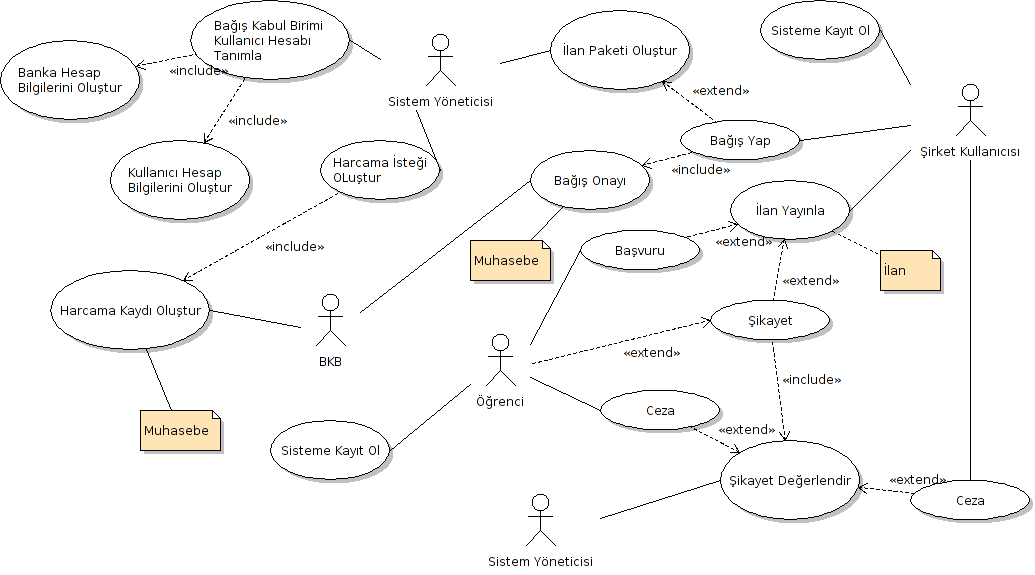
\includegraphics[width=.90\textwidth]{projectChapters/images/usecase.png}
    \caption{Kullanım Şeması}
    \label{ganttLabel}
\end{figure}

\section{Sınıf Diyagramı}
Kullanım şemasıyla belirlenen varlıklar ve eylemler, sınıf şemasında 1-1 ve 1-N ilişkiler ile gösterilmiştir. 
Bu ilişkiler bağlılık, parça-bütün ve kalıtım içermektedir. Projeye ait sınıf diyagramı Şekil 4.3'te incelenebilir.

\begin{figure}[]
    \centering
        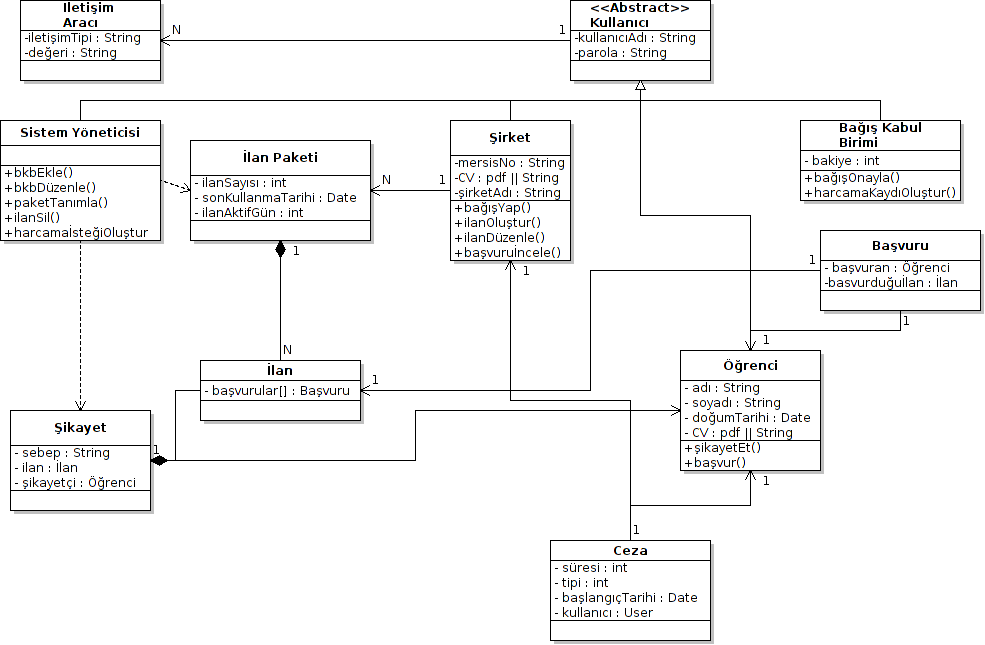
\includegraphics[width=.90\textwidth]{projectChapters/images/classUML.png}
    \caption{Sınıf Diyagramı}
    \label{ganttLabel}
\end{figure}


